\documentclass[notes,11pt, aspectratio=169, xcolor=table]{beamer}

\usepackage{pgfpages}
% These slides also contain speaker notes. You can print just the slides,
% just the notes, or both, depending on the setting below. Comment out the want
% you want.
\setbeameroption{hide notes} % Only slide
%\setbeameroption{show only notes} % Only notes
%\setbeameroption{show notes on second screen=right} % Both

\usepackage{helvet}
\usepackage[default]{lato}
\usepackage{array}

\newtheorem{proposition}{Proposition}
\newcommand{\blue}[1]{\textcolor{blue}{#1}}
\newcommand{\white}[1]{\textcolor{white}{#1}}

\usepackage{tikz}
\usetikzlibrary{shapes.geometric}
\usepackage{pgfplots}
\usetikzlibrary{patterns, pgfplots.fillbetween}
\usepackage{graphicx}
\usepackage{verbatim}
\setbeamertemplate{note page}{\pagecolor{yellow!5}\insertnote}
\usetikzlibrary{positioning}
\usetikzlibrary{snakes}
\usetikzlibrary{calc}
\usetikzlibrary{arrows}
\usetikzlibrary{decorations.markings}
\usetikzlibrary{shapes.misc}
\usetikzlibrary{matrix,shapes,arrows,fit,tikzmark}
\usepackage{amsmath}
\usepackage{mathpazo}
\usepackage{hyperref}
\usepackage{lipsum}
\usepackage{multimedia}
\usepackage{graphicx}
\usepackage{multirow}
\usepackage{graphicx}
\usepackage{dcolumn}
\usepackage{bbm}
\usepackage[style=authoryear,sorting=nyt,uniquename=false]{biblatex}

\addbibresource{references.bib} 

\newcolumntype{d}[0]{D{.}{.}{5}}

\def\@@mybluebox[#1][#2]#3{
    \sbox\mytempbox{#3}%
    \mytemplen\ht\mytempbox
    \advance\mytemplen #1\relax
    \ht\mytempbox\mytemplen
    \mytemplen\dp\mytempbox
    \advance\mytemplen #2\relax
    \dp\mytempbox\mytemplen
    \colorbox{myblue}{\hspace{1em}\usebox{\mytempbox}\hspace{1em}}}


\usepackage{changepage}
\usepackage{appendixnumberbeamer}
\newcommand{\beginbackup}{
   \newcounter{framenumbervorappendix}
   \setcounter{framenumbervorappendix}{\value{framenumber}}
   \setbeamertemplate{footline}
   {
     \leavevmode%
     \hline
     box{%
       \begin{beamercolorbox}[wd=\paperwidth,ht=2.25ex,dp=1ex,right]{footlinecolor}%
%         \insertframenumber  \hspace*{2ex} 
       \end{beamercolorbox}}%
     \vskip0pt%
   }
 }
\newcommand{\backupend}{
   \addtocounter{framenumbervorappendix}{-\value{framenumber}}
   \addtocounter{framenumber}{\value{framenumbervorappendix}} 
}


\usepackage{graphicx}
\usepackage[space]{grffile}
\usepackage{booktabs}

% These are my colors -- there are many like them, but these ones are mine.
\definecolor{blue}{RGB}{0,114,178}
\definecolor{red}{RGB}{213,94,0}
\definecolor{yellow}{RGB}{240,228,66}
\definecolor{green}{RGB}{0,158,115}

\hypersetup{
  colorlinks=false,
  linkbordercolor = {white},
  linkcolor = {blue}
}


%% I use a beige off white for my background
\definecolor{MyBackground}{RGB}{255,253,218}

%% Uncomment this if you want to change the background color to something else
%\setbeamercolor{background canvas}{bg=MyBackground}

%% Change the bg color to adjust your transition slide background color!
\newenvironment{transitionframe}{
  \setbeamercolor{background canvas}{bg=yellow}
  \begin{frame}}{
    \end{frame}
}

\setbeamercolor{frametitle}{fg=blue}
\setbeamercolor{title}{fg=blue}
\setbeamertemplate{footline}[frame number]
\setbeamertemplate{navigation symbols}{} 
\setbeamertemplate{itemize items}{-}
\setbeamercolor{itemize item}{fg=blue}
\setbeamercolor{itemize subitem}{fg=blue}
\setbeamercolor{enumerate item}{fg=blue}
\setbeamercolor{enumerate subitem}{fg=blue}
\setbeamercolor{button}{bg=MyBackground,fg=blue,}



% If you like road maps, rather than having clutter at the top, have a roadmap show up at the end of each section 
% (and after your introduction)
% Uncomment this is if you want the roadmap!
% \AtBeginSection[]
% {
%    \begin{frame}
%        \frametitle{Roadmap of Talk}
%        \tableofcontents[currentsection]
%    \end{frame}
% }
\setbeamercolor{section in toc}{fg=blue}
\setbeamercolor{subsection in toc}{fg=red}
\setbeamersize{text margin left=1em,text margin right=1em} 

\newenvironment{wideitemize}{\itemize\addtolength{\itemsep}{10pt}}{\enditemize}

\usepackage{environ}
\NewEnviron{videoframe}[1]{
  \begin{frame}
    \vspace{-8pt}
    \begin{columns}[onlytextwidth, T] % align columns
      \begin{column}{.58\textwidth}
        \begin{minipage}[t][\textheight][t]
          {\dimexpr\textwidth}
          \vspace{8pt}
          \hspace{4pt} {\Large \sc \textcolor{blue}{#1}}
          \vspace{8pt}
          
          \BODY
        \end{minipage}
      \end{column}%
      \hfill%
      \begin{column}{.42\textwidth}
        \colorbox{green!20}{\begin{minipage}[t][1.2\textheight][t]
            {\dimexpr\textwidth}
            Face goes here
          \end{minipage}}
      \end{column}%
    \end{columns}
  \end{frame}
}

\title[]{International Trade: Lecture 3}
\subtitle[]{Classical Ricardian Trade in General Equilibrium - Part I}
\author[Góes]
{Carlos Góes\inst{1}}
\date{Fall 2025}
\institute[GWU]{\inst{1} George Washington University }



\begin{document}

%%% TIKZ STUFF
\tikzset{   
        every picture/.style={remember picture,baseline},
        every node/.style={anchor=base,align=center,outer sep=1.5pt},
        every path/.style={thick},
        }
\newcommand\marktopleft[1]{%
    \tikz[overlay,remember picture] 
        \node (marker-#1-a) at (-.3em,.3em) {};%
}
\newcommand\markbottomright[2]{%
    \tikz[overlay,remember picture] 
        \node (marker-#1-b) at (0em,0em) {};%
}
\tikzstyle{every picture}+=[remember picture] 
\tikzstyle{mybox} =[draw=black, very thick, rectangle, inner sep=10pt, inner ysep=20pt]
\tikzstyle{fancytitle} =[draw=black,fill=red, text=white]
%%%% END TIKZ STUFF



%----------------------------------------------------------------------%
%-------------------       TITLE PAGE       ---------------------------%
%----------------------------------------------------------------------%





%----------------------------------------------------------------------%






%----------------------------------------------------------------------%
%----------------------------------------------------------------------%

%----------------------------------------------------------------------%
\frame{\titlepage}
\addtocounter{framenumber}{-1}
%----------------------------------------------------------------------%



%----------------------------------------------------------------------%
%----------------------------------------------------------------------%


\begin{frame}{Ricardian Model: Preliminaries}
\begin{wideitemize}
        \item 2  countries $i \in \{ US, COL\}$ and 2 products $p \in \{ C, R\}$
        \item In country $i$, there are $L_i$ units of labor (worker-hours) available 
        \item In country $i$, to produce one unit of good $p$, firms use $a_{i,p}$ units of labor
        \item \blue{Producers}: $\max_{Y_{i,p}} P_{i,p} Y_{i,p} - w_i a_{i,p} Y_{i,p}$ 
        \item \blue{PPF}: $a_{i,C} Y_{i,C} + a_{i,R} Y_{i,R} \le L_i$ 
        \item \blue{Preferences}: $Q_{i,C}^{\alpha_i} Q_{i,R}^{1-\alpha_i}$ 
        \end{wideitemize}
\end{frame}


\section{General}

\begin{frame}{General equilibrium}
\begin{wideitemize}
        \item Trade models are \blue{general equilibrium models}
        \item<2-> This means that \blue{prices will adjust} to achieve an equilibrium
        \item<3-> If supply exceeds demand for a given price, prices are ``too high''
        \item<4-> If demand exceeds supply for a given price,  prices are ``too low''
        \item<5-> It also means that we consider all markets together: the market for computers and roses affect each other...
        \item<6-> ... as does the market for factors of production (e.g., labor)
        \end{wideitemize}
\end{frame}

\begin{frame}{Production Technology}
\begin{wideitemize}
        \item In country $i$, firms producing good $p$ maximize profits under perfect competition:
        \begin{equation*}
            \max_{Y_{i,p}} \pi_{i,p} = \max_{Y_{i,p}} P_{i,p}Y_{i,p} - w_i a_{i,p} Y_{i,p} 
        \end{equation*}
        \item Since labor only one type of labor (mobile across sectors), there is a single wage $w_i$
        \item<3-> Total labor endowment satisfies the PPF across sectors:
        
        \begin{equation*}
            \underbrace{a_{i,C} \times Y_{i,C}}_{\substack{\text{labor used in} \\ \text{production of } C}} + \underbrace{a_{i,R} \times Y_{i,R}}_{\substack{\text{labor used in} \\ \text{production of } R}} \le \underbrace{L_i}_{\substack{\text{total labor} \\ \text{available in } i}}
        \end{equation*}

        \item<4-> In equilibrium, \textbf{prices equal marginal cost}:
        \begin{eqnarray*}
            P_{i,p} = w_i a_{i,p} \iff \frac{P_{i,p}}{a_{i,p}} = w_i  \qquad \text{ for } p \in\{C,R\}
        \end{eqnarray*}
    \end{wideitemize}
\end{frame}

\begin{frame}{Preferences}
\begin{wideitemize}
        \item In country $i$, consumers preferences over products $p$, represented by a utility function. 

        \begin{equation*}
            U_i(Q_C,Q_R) \equiv Q_C^{\alpha_i} Q_R^{1-\alpha_i}, \qquad \text{for } 0 < \alpha_i < 1   
        \end{equation*}
        \item<2-> Consumers take prices $P_{i,R},P_{i,C}$ as given and maximize: 
        \begin{equation*}
            \max_{\{Q_{i,C}, Q_{i,R}\}} U_i(Q_{i,C}, Q_{i,R}) \equiv Q_{i,C}^{\alpha_i} Q_{i,R}^{1-\alpha_i} \qquad s.t. \qquad P_{i,C} Q_{i,C} + P_{i,R} Q_{i,R} = w_i L_i
        \end{equation*}
        \item<3-> How to solve this?
        \end{wideitemize}
\end{frame}

\begin{frame}{Preferences}
\begin{wideitemize}
        \item<4> Rewrite budget constraint: $Q_{i,R} = \frac{w_i L_i}{P_{i,R}} - \frac{P_{i,C}}{P_{i,R} } Q_{i,C}$
        \item<2-> Replace in objective function and solve unconstrained max problem:

        \begin{equation*}
            \max_{\{Q_{i,C} \}} Q_C^{\alpha_i} \left( \frac{w_i L_i}{P_{i,R}} - \frac{P_{i,C}}{P_{i,R} } Q_{i,C} \right)^{1-\alpha_i}
        \end{equation*}
        \item<3-> First order condition: 
\scriptsize{
\begin{eqnarray*}
    & & \alpha_i Q_{i,C}^{\alpha_i-1} \left( \underbrace{\frac{w_i L_i}{P_{i,R}} - \frac{P_{i,C}}{P_{i,R} } Q_{i,C}}_{=Q_{i,R}} \right)^{1-\alpha_i} + Q_{i,C}^{\alpha_i} (1-\alpha_i) \left( \underbrace{\frac{w_i L_i}{P_{i,R}} - \frac{P_{i,C}}{P_{i,R} } Q_{i,C}}_{=Q_{i,R}} \right)^{1-\alpha_i-1} \left( - \frac{P_{i,C}}{P_{i,R}}\right) = 0 \\
%    & & \alpha_i  \left( \frac{Q_{i,R}}{Q_{i,C}} \right)^{1-\alpha_i} - (1-\alpha_i) \left( \frac{Q_{i,R}}{Q_{i,C}} \right)^{-\alpha_i} \left( \frac{P_{i,C}}{P_{i,R}}\right) = 0 \\
%    & & \alpha_i  \left( \frac{Q_{i,R}}{Q_{i,C}} \right)^{1-\alpha_i} = (1-\alpha_i) \left( \frac{Q_{i,R}}{Q_{i,C}} \right)^{-\alpha_i} \left( \frac{P_{i,C}}{P_{i,R}}\right) \\
%    & & \frac{Q_{i,R}}{Q_{i,C}}  = \frac{1-\alpha_i}{\alpha_i } \left( \frac{P_{i,C}}{P_{i,R}}\right) \\
\end{eqnarray*}
}
\normalsize
\begin{center}
    \boxed{$Q_{i,R}  = \frac{1-\alpha_i}{\alpha_i } \left( \frac{P_{i,C}}{P_{i,R}}\right) Q_{i,C}$}    
\end{center}

        \end{wideitemize}
\end{frame}

\begin{frame}{Preferences}
\begin{wideitemize}
        \item Replace result in budget constraint:

\scriptsize{
\begin{eqnarray*}
    Q_{i,R}&=& \frac{1-\alpha_i}{\alpha_i } \left( \frac{P_{i,C}}{P_{i,R}}\right) Q_{i,C}  = \frac{w_i L_i}{P_{i,R}} - \frac{P_{i,C}}{P_{i,R} } Q_{i,C} \\
    %\frac{1-\alpha_i}{\alpha_i } \left( \frac{P_{i,C}}{P_{i,R}}\right) Q_{i,C}  &=& \frac{w_i L_i}{P_{i,R}} - \frac{P_{i,C}}{P_{i,R} } Q_{i,C} \\
%    \frac{1-\alpha_i}{\alpha_i } \left( \frac{P_{i,C}}{P_{i,R}}\right) Q_{i,C} + \frac{P_{i,C}}{P_{i,R} } Q_{i,C} &=& \frac{w_i L_i}{P_{i,R}}  \\
%    \frac{1-\alpha_i + \alpha_i}{\alpha_i } \left( \frac{P_{i,C}}{P_{i,R}}\right) Q_{i,C} &=& \frac{w_i L_i}{P_{i,R}}  \\
\end{eqnarray*}
}

\normalsize
\begin{center}
    \boxed{$Q_{i,C} = \alpha_i  \frac{w_i L_i}{P_{i,C}}$}    
\end{center}


\item<2-> Finally:
{\scriptsize
\begin{eqnarray*}
     Q_{i,R}  &=& \frac{1-\alpha_i}{\alpha_i } \left( \frac{P_{i,C}}{P_{i,R}}\right) Q_{i,C}  = \frac{1-\alpha_i}{\alpha_i } \left( \frac{P_{i,C}}{P_{i,R}}\right) \alpha_i  \frac{w_i L_i}{P_{i,C}} \\
\end{eqnarray*}
}

\begin{center}
    \boxed{$Q_{i,R}  = (1-\alpha_i) \frac{w_i L_i}{P_{i,R}}$}    
\end{center}

\item<3-> Cobb-Douglas preferences: demand is a fixed share of their income $(\alpha_i, 1-\alpha_i)$; demand inversely proportional to the price of that good.
\item<4-> Holds regardless of whether consumers are in autarky or trade. 

\end{wideitemize}
\end{frame}

\section{Autarky Equilibrium}


\begin{frame}{Prices in Autarky Equilibrium}
\begin{wideitemize}
        \item In equilibrium, \textbf{prices equal marginal cost} in each productive sector:
        \begin{eqnarray*}
            P_{i,p} = w_i a_{i,p} \iff \frac{P_{i,p}}{a_{i,p}} = w_i  \qquad \text{ for } p \in\{C,R\}
        \end{eqnarray*}
        \item<2-> In autarky equilibrium, there demand and production in both sectors
        \item We can pin down the relative price $P_{i,C} / P_{i,R}$:
        \begin{center}
        \boxed{
            \frac{P_{i,C}}{a_{i,C}} = w_i = \frac{P_{i,R}}{a_{i,R}} \iff \frac{P_{i,C}}{P_{i,R}} = \frac{a_{i,C}}{a_{i,R}}  
        }            
        \end{center}
    \item<3-> In autarky, relative prices will reflect the \textbf{opportunity cost} within country $i$

\end{wideitemize}
\end{frame}

\begin{frame}{Autarky Equilibrium}
\begin{wideitemize}
    \item Replacing $\frac{P_{i,p}}{a_{i,p}} = w_i \iff P_{i,C} = w_i a_{i,p}$ in demand functions solves in terms of parameters:
\begin{center}
    \boxed{$Q_{i,C} = \alpha_i  \frac{w_i L_i}{P_{i,C}}=  \alpha_i  \frac{L_i}{a_{i,C}} ,\qquad Q_{i,R}  = (1-\alpha_i) \frac{w_i L_i}{P_{i,R}} = (1-\alpha_i) \frac{L_i}{a_{i,R}}$}    
\end{center}
    \item<2-> In equilibrium, \blue{supply equals demand}:

    \begin{center}
    \boxed{$Y_{i,C} = Q_{i,C},\qquad Y_{i,R} = Q_{i,R}$}    
\end{center}

    \item<4-> We have solved for optimal demands $( Q_{i,C}, Q_{i,R})$, get $(Y_{i,C}, Y_{i,R})$   ``for free''
    \item<5->  Can check choices satisfy the PPF:
    {\scriptsize
        \begin{eqnarray*}
            a_{i,C} \times Y_{i,C} + a_{i,R} \times Y_{i,R} &=& L_i \\
            a_{i,C} \times Q_{i,C} + a_{i,R} \times Q_{i,R} &=& L_i \qquad (\text{mkt clearing}) \\
            a_{i,C} \times \alpha_i  \frac{L_i}{a_{i,C}} + a_{i,R} \times (1-\alpha_i) \frac{L_i}{a_{i,R}}  &=& L_i \qquad (\text{optimal demand}) \\
            \alpha_i  L_i + (1-\alpha_i) L_i  &=& L_i \qquad (\text{checks out!})
        \end{eqnarray*}
        }
\end{wideitemize}
\end{frame}

\begin{frame}{Numerical example: Autarky}
\centering
\resizebox{\textwidth}{!}{%
\begin{tabular}{lcc}
\toprule
\textbf{Variable} & \textbf{United States (US)} & \textbf{Colombia (COL)} \\
\midrule
Labor endowment $L_i$ & $300$ million & $54$ million \\
Preference parameter $\alpha_i$ & $1/2$ & $3/4$ \\
Unit labor requirement for computers $a_{i,C}$ & $3{,}000$ & $5{,}400$ \\
Unit labor requirement for roses $a_{i,R}$ & $30$ & $6$ \\
\midrule
Max computers: $L_i / a_{i,C}$ & \white{$300\text{m}/3{,}000 = 100{,}000$} & \white{$54\text{m}/5{,}400 = 10{,}000$} \\
Max roses: $L_i / a_{i,R}$ & \white{$300\text{m}/30 = 10\text{m}$} & \white{$54\text{m}/6 = 9\text{m}$} \\
\midrule
Opportunity cost $a_{i,C}/a_{i,R}$ & \white{$3{,}000/30 = 100$} & \white{$5{,}400/6 = 900$} \\
Demand for computers: $\alpha_i L_i / a_{i,C}$ & \white{$0.5 \times 300\text{m}/3{,}000 = 50{,}000$} & \white{$0.75 \times 54\text{m}/5{,}400 = 7{,}500$} \\
Demand for roses: $(1{-}\alpha_i) L_i / a_{i,R}$ & \white{$0.5 \times 300\text{m}/30 = 5\text{m}$} & \white{$0.25 \times 54\text{m}/6 = 2.25\text{m}$} \\
\bottomrule
\end{tabular}
}
\end{frame}

\begin{frame}{Numerical example: Autarky}
\addtocounter{framenumber}{-1}

\centering
\resizebox{\textwidth}{!}{%
\begin{tabular}{lcc}
\toprule
\textbf{Variable} & \textbf{United States (US)} & \textbf{Colombia (COL)} \\
\midrule
Labor endowment $L_i$ & $300$ million & $54$ million \\
Preference parameter $\alpha_i$ & $1/2$ & $3/4$ \\
Unit labor requirement for computers $a_{i,C}$ & $3{,}000$ & $5{,}400$ \\
Unit labor requirement for roses $a_{i,R}$ & $30$ & $6$ \\
\midrule
Max computers: $L_i / a_{i,C}$ & $300\text{m}/3{,}000 = 100{,}000$ & $54\text{m}/5{,}400 = 10{,}000$ \\
Max roses: $L_i / a_{i,R}$ & $300\text{m}/30 = 10\text{m}$ & $54\text{m}/6 = 9\text{m}$ \\
\midrule
Opportunity cost $a_{i,C}/a_{i,R}$ & \white{$3{,}000/30 = 100$} & \white{$5{,}400/6 = 900$} \\
Demand for computers: $\alpha_i L_i / a_{i,C}$ & \white{$0.5 \times 300\text{m}/3{,}000 = 50{,}000$} & \white{$0.75 \times 54\text{m}/5{,}400 = 7{,}500$} \\
Demand for roses: $(1{-}\alpha_i) L_i / a_{i,R}$ & \white{$0.5 \times 300\text{m}/30 = 5\text{m}$} & \white{$0.25 \times 54\text{m}/6 = 2.25\text{m}$} \\
\bottomrule
\end{tabular}
}
\end{frame}

\begin{frame}{Numerical example: Autarky}
\addtocounter{framenumber}{-1}
\centering
\resizebox{\textwidth}{!}{%
\begin{tabular}{lcc}
\toprule
\textbf{Variable} & \textbf{United States (US)} & \textbf{Colombia (COL)} \\
\midrule
Labor endowment $L_i$ & $300$ million & $54$ million \\
Preference parameter $\alpha_i$ & $1/2$ & $3/4$ \\
Unit labor requirement for computers $a_{i,C}$ & $3{,}000$ & $5{,}400$ \\
Unit labor requirement for roses $a_{i,R}$ & $30$ & $6$ \\
\midrule
Max computers: $L_i / a_{i,C}$ & $300\text{m}/3{,}000 = 100{,}000$ & $54\text{m}/5{,}400 = 10{,}000$ \\
Max roses: $L_i / a_{i,R}$ & $300\text{m}/30 = 10\text{m}$ & $54\text{m}/6 = 9\text{m}$ \\
\midrule
Opportunity cost $a_{i,C}/a_{i,R}$ & $3{,}000/30 = 100$ & $5{,}400/6 = 900$ \\
Demand for computers: $\alpha_i L_i / a_{i,C}$ & $0.5 \times 300\text{m}/3{,}000 = 50{,}000$ & $0.75 \times 54\text{m}/5{,}400 = 7{,}500$ \\
Demand for roses: $(1{-}\alpha_i) L_i / a_{i,R}$ & $0.5 \times 300\text{m}/30 = 5\text{m}$ & $0.25 \times 54\text{m}/6 = 2.25\text{m}$ \\
\bottomrule
\end{tabular}
}
\end{frame}

\begin{frame}{Autarky Equilibrium}
\begin{figure}[htbp!]

% California
\begin{subfigure}{}
\resizebox{0.48\textwidth}{!}{%
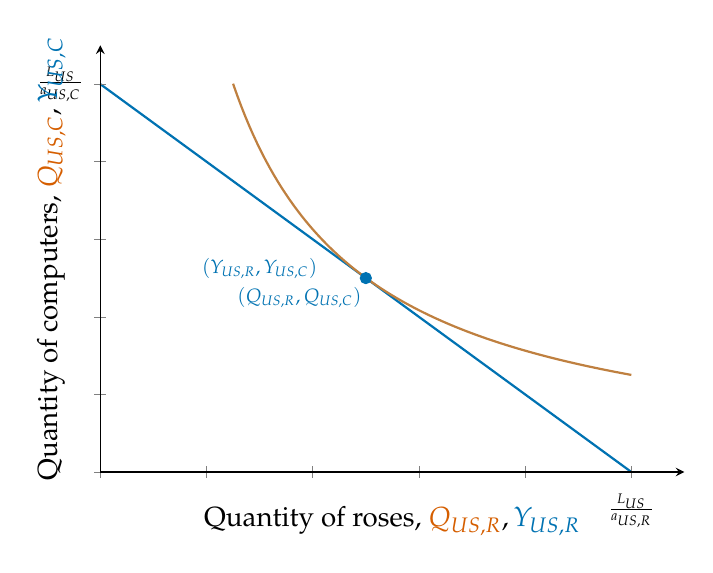
\begin{tikzpicture}
\pgfmathsetmacro{\aC}{100}       % unit labor requirement for computers
\pgfmathsetmacro{\aR}{1}         % unit labor requirement for roses
\pgfmathsetmacro{\alpha}{0.5}    % preference for computers
\pgfmathsetmacro{\Lendow}{10}    % labor endowment

% Compute equilibrium quantities
\pgfmathsetmacro{\Qc}{(\alpha*\Lendow)/\aC}
\pgfmathsetmacro{\Qr}{((1 - \alpha)*\Lendow)/\aR}

% Compute utility level
\pgfmathsetmacro{\U}{(\Qc^(\alpha))*(\Qr^(1 - \alpha))}

% Compute prefactor for indifference curve: Qc = A * Qr^(- (1 - alpha)/alpha)
\pgfmathsetmacro{\expo}{(1 - \alpha)/\alpha}
\pgfmathsetmacro{\A}{\U^(1/\alpha)}

\centering
\begin{axis}[
    ylabel={Quantity of computers, $\textcolor{red}{Q_{US,C}}, \textcolor{blue}{Y_{US,C}}$},
    xlabel={Quantity of roses, $\textcolor{red}{Q_{US,R}}, \textcolor{blue}{Y_{US,R}}$},
    ymin=0, ymax=0.11,
    xmin=0, xmax=11,
    yticklabel=\empty,
    xticklabel=\empty,
    axis lines=left,
    enlargelimits=false,
    clip=false,
    axis on top,
    scaled x ticks=false,
    width=9cm, height=7cm,
    title style={font=\bfseries}
]

% PPF: Q_C = (L/a_C) - (a_R/a_C) * Q_R
\addplot[thick, blue, domain=0:10] {\Lendow/\aC - (\aR/\aC)*x};

% Indifference curve through optimal bundle
\addplot[thick, brown, domain=2.5:10, samples=100] {\A * x^(-\expo)};

% Labels
%\node at (axis cs:3.5,0.03) {\Large $\mathcal{Y}_{US}$};
\node at (axis cs:\Lendow/\aR,-.01) {\scriptsize $\frac{L_{US}}{a_{US,R}}$};
\node at (axis cs:-.75,\Lendow/\aC) {\scriptsize $\frac{L_{US}}{a_{US,C}}$};


% Equilibrium point
\addplot[only marks, mark=*, color=blue, mark size=2pt] coordinates {(\Qr, \Qc)};
\node at (axis cs:\Qr - 1.25,\Qc - 0.005) {\scriptsize $\textcolor{blue}{(Q_{US,R},Q_{US,C})}$};
\node at (axis cs:\Qr - 2,\Qc + 0.0025) {\scriptsize $\textcolor{blue}{(Y_{US,R},Y_{US,C})}$};



\end{axis}

\end{tikzpicture}
}
\end{subfigure}
%
% Colombia
\begin{subfigure}{}
\resizebox{0.48\textwidth}{!}{%

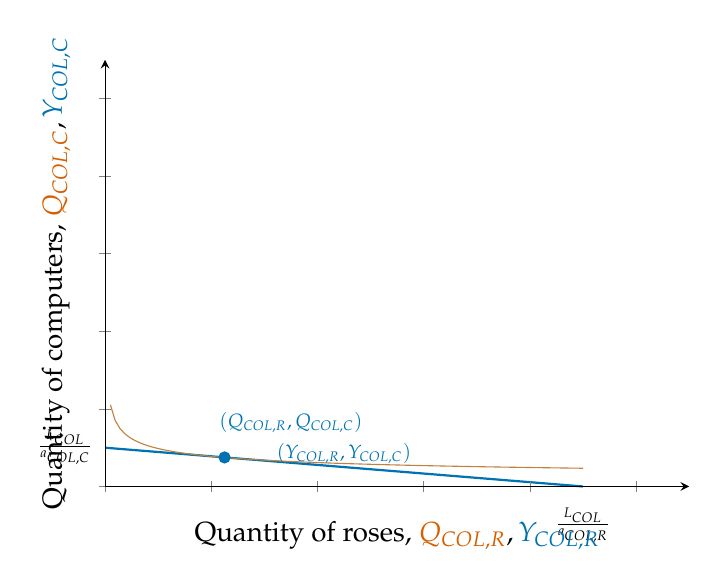
\begin{tikzpicture}
\pgfmathsetmacro{\aC}{900}       % unit labor requirement for computers
\pgfmathsetmacro{\aR}{1}         % unit labor requirement for roses
\pgfmathsetmacro{\alpha}{0.75}    % preference for computers
\pgfmathsetmacro{\Lendow}{9}    % labor endowment

% Compute equilibrium quantities
\pgfmathsetmacro{\Qc}{(\alpha*\Lendow)/\aC}
\pgfmathsetmacro{\Qr}{((1 - \alpha)*\Lendow)/\aR}

% Compute utility level
\pgfmathsetmacro{\U}{(\Qc^(\alpha))*(\Qr^(1 - \alpha))}

% Compute prefactor for indifference curve: Qc = A * Qr^(- (1 - alpha)/alpha)
\pgfmathsetmacro{\expo}{(1 - \alpha)/\alpha}
\pgfmathsetmacro{\A}{\U^(1/\alpha)}

\centering
\begin{axis}[
    ylabel={Quantity of computers, $\textcolor{red}{Q_{COL,C}}, \textcolor{blue}{Y_{COL,C}}$},
    xlabel={Quantity of roses, $\textcolor{red}{Q_{COL,R}}, \textcolor{blue}{Y_{COL,R}}$},
    ymin=0, ymax=0.11,
    xmin=0, xmax=11,
    yticklabel=\empty,
    xticklabel=\empty,
    axis lines=left,
    enlargelimits=false,
    clip=false,
    axis on top,
    scaled x ticks=false,
    width=9cm, height=7cm,
    title style={font=\bfseries}
]

% PPF: Q_C = (L/a_C) - (a_R/a_C) * Q_R
\addplot[thick, blue, domain=0:9] {\Lendow/\aC - (\aR/\aC)*x};

% Indifference curve through optimal bundle
\addplot[brown, domain=0.1:9, samples=100] {\A * x^(-\expo)};

% Labels

%\node at (axis cs:3.5,0.03) {\Large $\mathcal{Y}_{US}$};
\node at (axis cs:\Lendow/\aR,-.01) {\scriptsize $\frac{L_{COL}}{a_{COL,R}}$};
\node at (axis cs:-.75,\Lendow/\aC) {\scriptsize $\frac{L_{COL}}{a_{COL,C}}$};


% Equilibrium point
\addplot[only marks, mark=*, color=blue, mark size=2pt] coordinates {(\Qr, \Qc)};
\node at (axis cs:\Qr + 1.25,\Qc + 0.009) {\scriptsize $\textcolor{blue}{(Q_{COL,R},Q_{COL,C})}$};
\node at (axis cs:\Qr + 2.25,\Qc + 0.001) {\scriptsize $\textcolor{blue}{(Y_{COL,R},Y_{COL,C})}$};


\end{axis}

\end{tikzpicture}
}

\end{subfigure}

\caption{Autarky equilibrium}\label{fig: autarky-num}

\end{figure}

\end{frame}

\end{document}
